\documentclass[tikz,margin=0.5cm]{standalone}

\usetikzlibrary{decorations.text}

\begin{document}
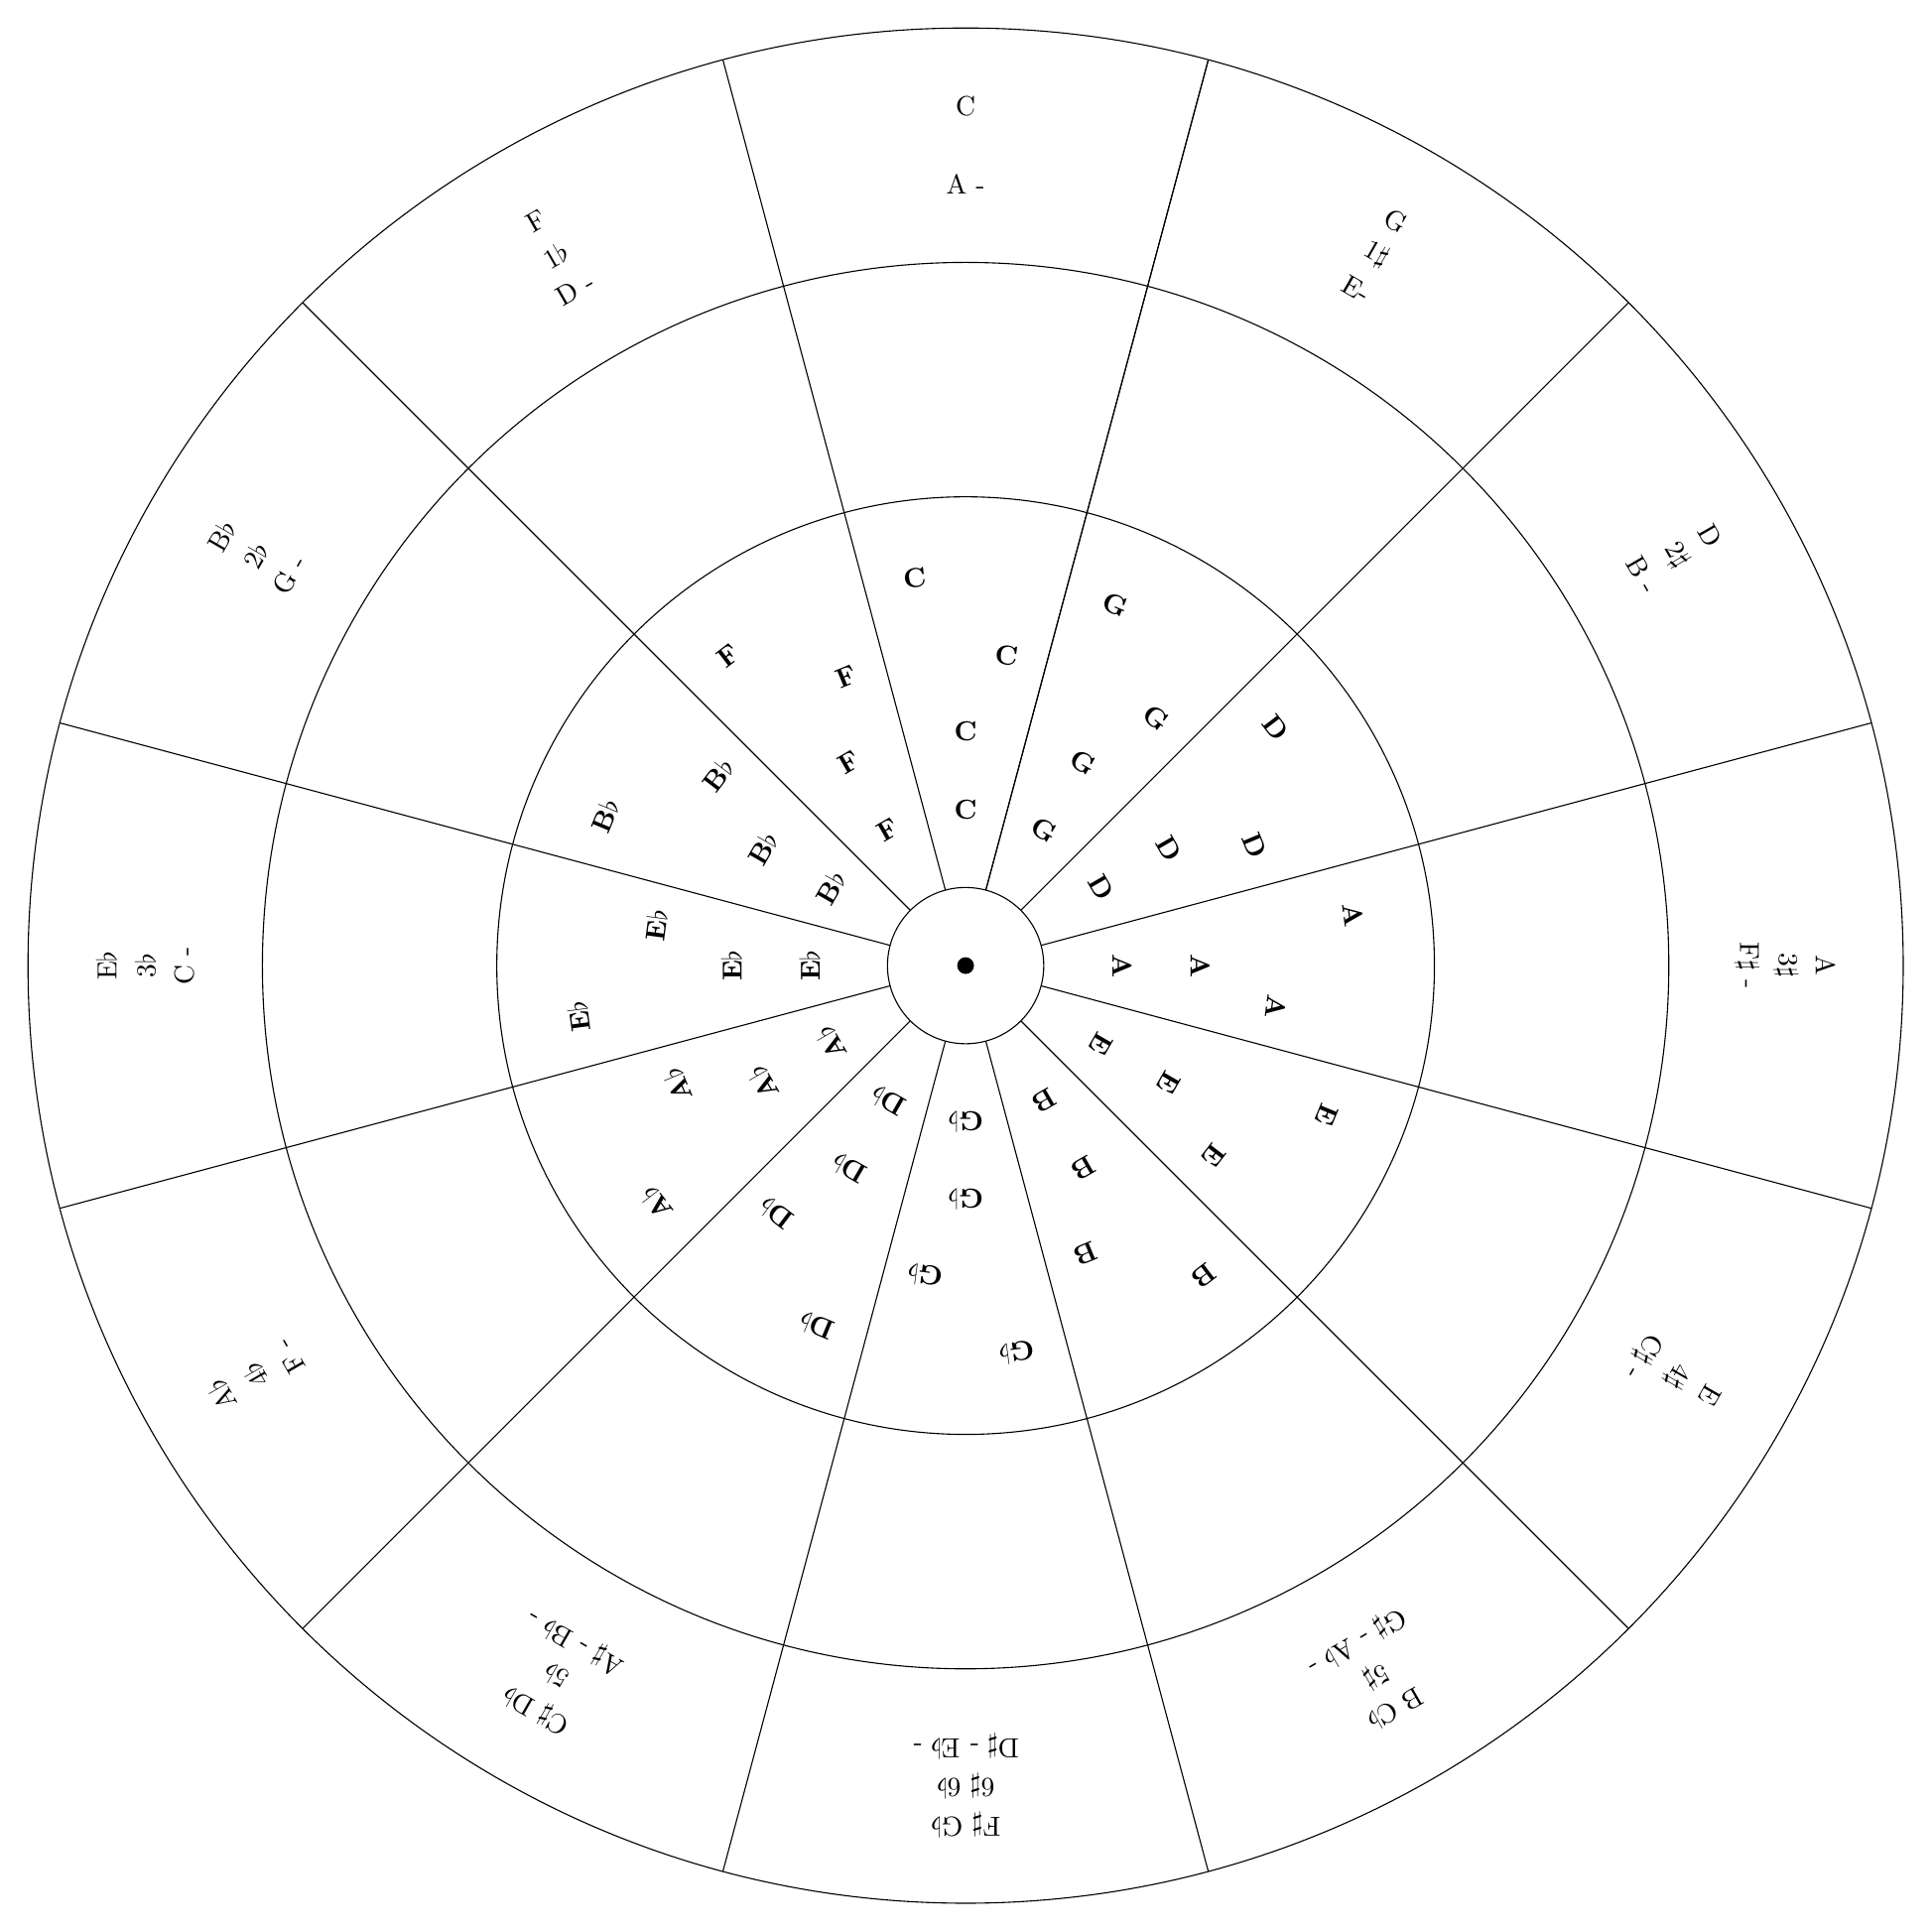
\begin{tikzpicture}

\pgfmathsetmacro{\CircROne}{12}
\pgfmathsetmacro{\CircRTwo}{9}
\pgfmathsetmacro{\CircRThree}{6}
\pgfmathsetmacro{\MajorR}{11}
\pgfmathsetmacro{\ScaleR}{10.5}
\pgfmathsetmacro{\MinorR}{10}
\pgfmathsetmacro{\DegreeR}{8.25}
\pgfmathsetmacro{\ExtR}{7.75}
\pgfmathsetmacro{\ModeR}{7.25}
\pgfmathsetmacro{\ModernR}{6.75}
\pgfmathsetmacro{\ChordsR}{5}

% THE GRID
\draw (0,0) circle (\CircROne);
\draw (0,0) circle (\CircRTwo);
\draw (0,0) circle (\CircRThree);
\foreach \X in {0,1,...,12}
    {
    \draw (0,0)--++(75-\X*360/12:\CircROne);
    }
\draw [fill=white] (0,0) circle (1cm);
\draw [fill=black] (0,0) circle (1mm);

%%%Scale 

%%% Phase 1, Base plate: enable this!
%%% Phase 2, Degree plate: enable this!
%%% Phase 3, Chord plate: enable this!
%%% Example: enable this! 
%%% Example with colors: enable this!

\foreach \X/\Major/\Minor/\Scale in {
-5/{C$\sharp$ D$\flat$}/{A$\sharp$~- B$\flat$~-}/5$\flat$,
-4/A$\flat$/F~-/4$\flat$,
-3/E$\flat$/C~-/3$\flat$,
-2/B$\flat$/G~-/2$\flat$,
-1/F/D~-/1$\flat$,
0/C/A~-/{},
1/G/E-/1$\sharp$,
2/D/B~-/2$\sharp$,
3/A/F$\sharp$~-/3$\sharp$,
4/E/C$\sharp$~-/4$\sharp$,
5/{B C$\flat$}/{G$\sharp$~- A$\flat$~-}/5$\sharp$,
6/{F$\sharp$ G$\flat$}/{D$\sharp$~- E$\flat$~-}/{6$\sharp$ 6$\flat$}}
    {
    \draw (90-\X*360/12:\MajorR) node [align=left, rotate=-\X*360/12] {\Major};
    \draw (90-\X*360/12:\ScaleR) node [align=left, rotate=-\X*360/12] {\Scale};
    \draw (90-\X*360/12:\MinorR) node [align=center, rotate=-\X*360/12] {\Minor};
    }

%%%Scale end

%%%Chord notes

%%% Phase 1, Base plate: enable this!
%%% Phase 2, Degree plate: disable this!
%%% Phase 3, Chord plate: disable this!
%%% Example: disable this! 
%%% Example with colors: disable this!

\foreach \Note/\X in {C/0,G/1,D/2,A/3,E/4,B/5,G$\flat$/6,D$\flat$/-5,A$\flat$/-4,E$\flat$/-3,B$\flat$/-2,F/-1}
    {
    \foreach \dX/\Y in {-0.25/\ChordsR,0.25/{\ChordsR-1},0/{\ChordsR-2},0/{\ChordsR-3}}
        {
        \pgfmathsetmacro{\rX}{\X+\dX}
        \draw(90-\rX*360/12:\Y) node [align=center, rotate=-\rX*360/12] {\textbf{\Note}};
        }
    }

%%%Chord notes end

%%%Degree

%%% Phase 1, Base plate: disable this!
%%% Phase 2, Degree plate: enable this!
%%% Phase 3, Chord plate: disable this!
%%% Example: enable this, but disable line with "cut this"!
%%% Example with colors: enable this, but disable line with "cut this" and add "text=blue" to \Mode and "text=red" to \Modern!

% \foreach \X/\Degree/\Mode/\Ext/\Modern in {
% 0/I$\triangle$/ionian/{}/major,
% -2/ii7/dorian/9/{},
% -4/iii7/phrygian/{}/{},
% 1/IV$\triangle$/lydian/11/{},
% -1/V7/mixolydian/{}/{},
% -3/vi7/aeolian/13/{natural minor},
% -5/vii{\o}/locrian/{}/{}}
%     {
%     \draw (90+\X*360/12:\DegreeR) node[align=center, rotate=\X*360/12] {\Degree};
%     \draw (90+\X*360/12:\ExtR) node[align=center, rotate=\X*360/12] {\Ext};
%     \draw (90+\X*360/12:\ModeR) node[align=center, rotate=\X*360/12] {\Mode};
%     % \draw (90+\X*360/12:\ModeR) node[align=center, text=blue,rotate=\X*360/12] {\Mode};
%     \draw (90+\X*360/12:\ModernR) node[align=center, rotate=\X*360/12] {\Modern};
%     % \draw (90+\X*360/12:\ModernR) node[align=center, text=red,rotate=\X*360/12] {\Modern};
%     \draw (90+\X*360/12:5) node {cut this};
%     }

%%%Modes end

%%%Chords

%%% Phase 1, Base plate: disable this!
%%% Phase 2, Degree plate: disable this!
%%% Phase 3, Chord plate: enable this!
%%% Example: enable this!
%%% Example with colors: enable this!

% % root
% \pgfmathsetmacro{\rootX}{-0.25}
% \pgfmathsetmacro{\rootY}{\ChordsR}
% \pgfmathsetmacro{\rootlblX}{\rootX+0.20}
% \pgfmathsetmacro{\rootlblY}{\rootY-0.45}
% \pgfmathsetmacro{\rootlbl}{1}
% % third (2x)
% \pgfmathsetmacro{\thirdAX}{4+0.25}
% \pgfmathsetmacro{\thirdBX}{-3+0.25}
% \pgfmathsetmacro{\thirdY}{\ChordsR-1}
% \pgfmathsetmacro{\thirdAlblX}{\thirdAX-0.30}
% \pgfmathsetmacro{\thirdBlblX}{\thirdBX-0.30}
% \pgfmathsetmacro{\thirdAlblY}{\thirdY-0.2}
% \pgfmathsetmacro{\thirdBlblY}{\thirdY-0.2}
% \pgfmathsetmacro{\thirdlbl}{3}
% % fifth
% \pgfmathsetmacro{\fifthX}{1}
% \pgfmathsetmacro{\fifthY}{\ChordsR-2}
% \pgfmathsetmacro{\fifthlblX}{\fifthX-0.35}
% \pgfmathsetmacro{\fifthlblY}{\fifthY+0.35}
% \pgfmathsetmacro{\fifthlbl}{5}
% % seventh (2x)
% \pgfmathsetmacro{\seventhAX}{5}
% \pgfmathsetmacro{\seventhBX}{-2}
% \pgfmathsetmacro{\seventhY}{\ChordsR-3}
% \pgfmathsetmacro{\seventhAlblX}{\seventhAX-0.3}
% \pgfmathsetmacro{\seventhBlblX}{\seventhBX+0.3}
% \pgfmathsetmacro{\seventhAlblY}{\seventhY+0.55}
% \pgfmathsetmacro{\seventhBlblY}{\seventhY+0.55}
% \pgfmathsetmacro{\seventhlbl}{7}

% \foreach \X/\Y/\lblX/\lblY/\lbl in {
% \rootX/\rootY/\rootlblX/\rootlblY/\rootlbl,
% \thirdAX/\thirdY/\thirdAlblX/\thirdAlblY/\thirdlbl,
% \thirdBX/\thirdY/\thirdBlblX/\thirdBlblY/\thirdlbl,
% \fifthX/\fifthY/\fifthlblX/\fifthlblY/\fifthlbl,
% \seventhAX/\seventhY/\seventhAlblX/\seventhAlblY/\seventhlbl,
% \seventhBX/\seventhY/\seventhBlblX/\seventhBlblY/\seventhlbl}
%     {
%     \draw (90-\X*360/12:\Y) node [circle,draw,minimum size =2.5em] {};
%     \draw (90-\lblX*360/12:\lblY) node[align=center, rotate=-\lblX*360/12] {\lbl};
%     }

% \draw [-stealth,ultra thick] (0,\ChordsR) -- (0,\CircRThree);
% \draw (90-6*360/12:\ChordsR ) node [align=center, rotate=-6*360/12] {add\\to\\vii{\o}\\(5)};

%%%Chords end

%%%Example

%%% Phase 1, Base plate: disable this!
%%% Phase 2, Degree plate: disable this!
%%% Phase 3, Chord plate: disable this!
%%% Example: enable this!
%%% Example with colors: enable this!

% \foreach \Note/\X/\Y in {C/\rootX/\rootY,G/\fifthX/\fifthY,E/\thirdAX/\thirdY,B/\seventhAX/\seventhY}
%     {
%     \draw(90-\X*360/12:\Y) node [circle,draw=black,minimum size=2.5em,fill=gray, fill opacity=0.2,text opacity=1,align=center, rotate=-\X*360/12] {\Note};
%     }

%%%Example end

%%%Example with colors

%%% Phase 1, Base plate: disable this!
%%% Phase 2, Degree plate: disable this!
%%% Phase 3, Chord plate: disable this!
%%% Example: disable this!
%%% Example with colors: enable this!

% \draw[draw=none,fill=green,fill opacity=0.2,even odd rule]  (0,0) circle (\MajorR+0.25) (0,0) circle (\MajorR-0.25);
% \draw[draw=none,fill=yellow,fill opacity=0.2,even odd rule]  (0,0) circle (\ScaleR+0.25) (0,0) circle (\ScaleR-0.25);
% \draw[draw=none,fill=red,fill opacity=0.2,even odd rule]  (0,0) circle (\MinorR+0.25) (0,0) circle (\MinorR-0.25);
% \draw[draw=none,fill=blue,fill opacity=0.2,even odd rule]  (0,0) circle (\DegreeR+0.25) (0,0) circle (\DegreeR-0.25);
% \draw[draw=none,fill=orange,fill opacity=0.2,even odd rule]  (0,0) circle (\ExtR+0.25) (0,0) circle (\ExtR-0.25);

%%%Example with colors end

\end{tikzpicture}
\end{document}